\chapter{Introduction}
\section{Machine Translation}
    \justify
    \textbf{Machine Translation}, which is also abbreviated by \textbf{MT} is an important problem of Natural Language Processing (NLP). It can be defined as- \say{the translation of human language by a machine}. The machines are trained in such a way that, during testing, it can translate any text from a \textit{source language} to \textit{target language}. \textit{Source language} is the language in which a text is already written; while \textit{target language} is the language in which text has to be translated. 
    
\section{History of Machine Translation}
    The current \textit{state-of-art} MT researchers have made very sophisticated MT systems capable of translating a text with very good accuracy, giving almost 100\% knowledge about the sentence. But the main research in the field MT began in 1950s. \textbf{The Georgetown Experiment}\cite{MThistory} was the earliest MT experiment, which involved translating 60 Russian sentences into English. 
    
    The earlier systems consisted of a bilingual dictionary which had a mapping for each word from source language to target language and set of rules to predict word order once all words were mapped. This systems were too constrained in the sense that they were language specific, rules change as the target or source language change, the rules were not even consistent as there were always sentences which didn't follow the grammar rules. There was a clear lack of semantic rules which could actually grasp the meaning of sentence. Researchers in time couldn't find specific solutions for such problems. This led to the shutting down funding in the research of MT by ALPAC committee\cite{MThistory} in 1964 formed by US government. 
    
    The 1980s and 90s saw the rise of many MT based systems namely \textbf{Systran} and \textbf{Logos}, which translated text to/from German, Russian and other European languages. Several Example Based Systems were also developed in the same period, in which for each source sentence, the most similar sentence in target language was found in parallel corpus. Meanwhile, data driven methods began popularity. IBM began its research in MT with a more specific term called as \textbf{Statistical Machine Translation}. Currently, SMT is one of the most sutdied MT method. Various IBM model were released sequentially to overcome the drawback of previous models. Later on an MT engine based on SMT called \textbf{Moses} was also released. 
    
    \begin{figure}
        \centering
        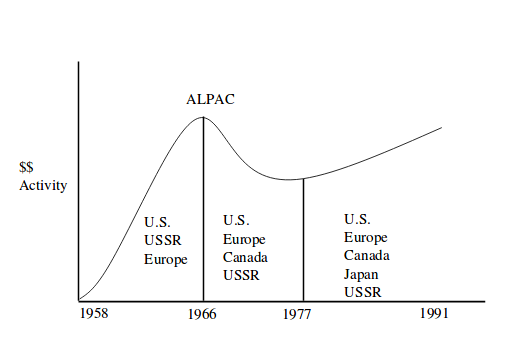
\includegraphics[scale=0.6]{Images/mtHistory.png}
        \caption{History of MT}
        \label{fig:history}
    \end{figure}
    The state-of-the art method used primarily in MT is Neural Machine Translation, which uses Neural Networks to encode source sentences to decode in target sentences. Currently, an open source Neural Networks based Machine Translation system is developed by Harvard known as OpenNMT\cite{openNMT}.
        
\section{Paradigms of Machine Translation}
    The three main paradigms of Machine Translation are Rule Based Machine Translation, Statistical Machine Translation and Example Based Machine Translation. The main goal of all the paradigms are the same, i.e. to translate a text from source to target language. However, all the paradigms differ in the methodology of translating. Each paradigm has its own pros and cons of using it, like the domain, cost to build such a system, time to build and most importantly the accuracy of the translation.
    
    \subsection{Rule Based Machine Translation}
    \textbf{Rule Based Machine Translation} or more commonly known as \textbf{RBMT} is a traditional paradigm of machine translation. It uses the linguistic information of the language to create rules using which it helps in translation. Since the whole idea of translation in this paradigm is based on rules of language, hence rules should be carefully written. Rules are written by linguistic experts of languages which are involved in translation. All the diverse phenomenon should be covered by rules of the translation. 
    
    Rule based MT incurs huge time and effort. Each phenomena of the language has to be captured which is generally not possible. Rule based MT often suffers from high precision and low recall problem, i.e. the system will perform good on seen data since seeing them rules are written by the expert, but will perform poorly on unseen data. The diverse language regularities and constraints are often uncovered by rules.
    
    \subsection{Statistical Machine Translation}
    \textbf{Statistical Machine Translation} or \textbf{SMT} is a data-driven method of Machine Translation. Unlike RBMT, there are no rules in SMT, instead a thorough statistical analysis of parallel corpora has to be done. IBM began research in SMT, developing various SMT models called as the IBM models. Each model captures a distinct feature of language and overcomes drawbacks of previous models. 
    
    Statistical Machine Translation does translation by capturing probabilities of two models, namely \textbf{Translational Model} and \textbf{Language Model}. Translational models gives the probability of how likely is the target sentence given source sentence, which is often broken down to word level. Language model gives the probability of how probable is the translated target language sentence with respect to fluency and adequacy in the context of target language sentence. Both these probabilities are combined to form a noisy-channel model which predicts the most probable sentence from a source language sentence.
    
    \subsection{Example Based Machine Translation}
    \textbf{Example Baed Machine Translation} or \textbf{EMBT} is another paradigm of machine translation. It was introduced in 1980s. 
    
    EBMT is also a data-driven method, it heavily depends on parallel corpora. A source language sentence is searched in the parallel corpora to find best possible matching sentence in source language. If an exact match is found, then its translation in the target language which is also stored in parallel corpora is returned. But if no exact match is found, best possible matching sentence is taken and it's translation is returned with slight modifications to the translation to adapt the changes. Sometimes two or more sentence are matched in parts, and their translations are returned and joined in similar fashion to return one single translation of the source sentence. 
    
    
